
\section{System Design}

!!The state transition matrix phi[K,W,W] is trained offline via simple MLE (counting transitions), completely separate from the neural network.


We illustrate the pipeline of \ac{tfow} in \autoref{fig:pipeline}, which is composed of three key modules: 
\begin{enumerate*}[label={(\roman*)}]
    \item data collector;
    \item event constructor;
    \item anomaly detector. 
\end{enumerate*}
The data collector gathers trades and limit order book updates, which are then transformed by the event constructor into a sequence of order events. These sequences serve as inputs to the anomaly detector, which first identifies abnormal sequences using the sum-of-squared-spacings statistic, and subsequently localizes the anomalies via hitting-time and A-before-B query queries. Note, the anomaly detector starts by raising deviation alerts at the sequence level, and then pinpoints anomalies at timestamps and uncovers the underlying temporal motifs.
\begin{figure}[!h]
  \centering  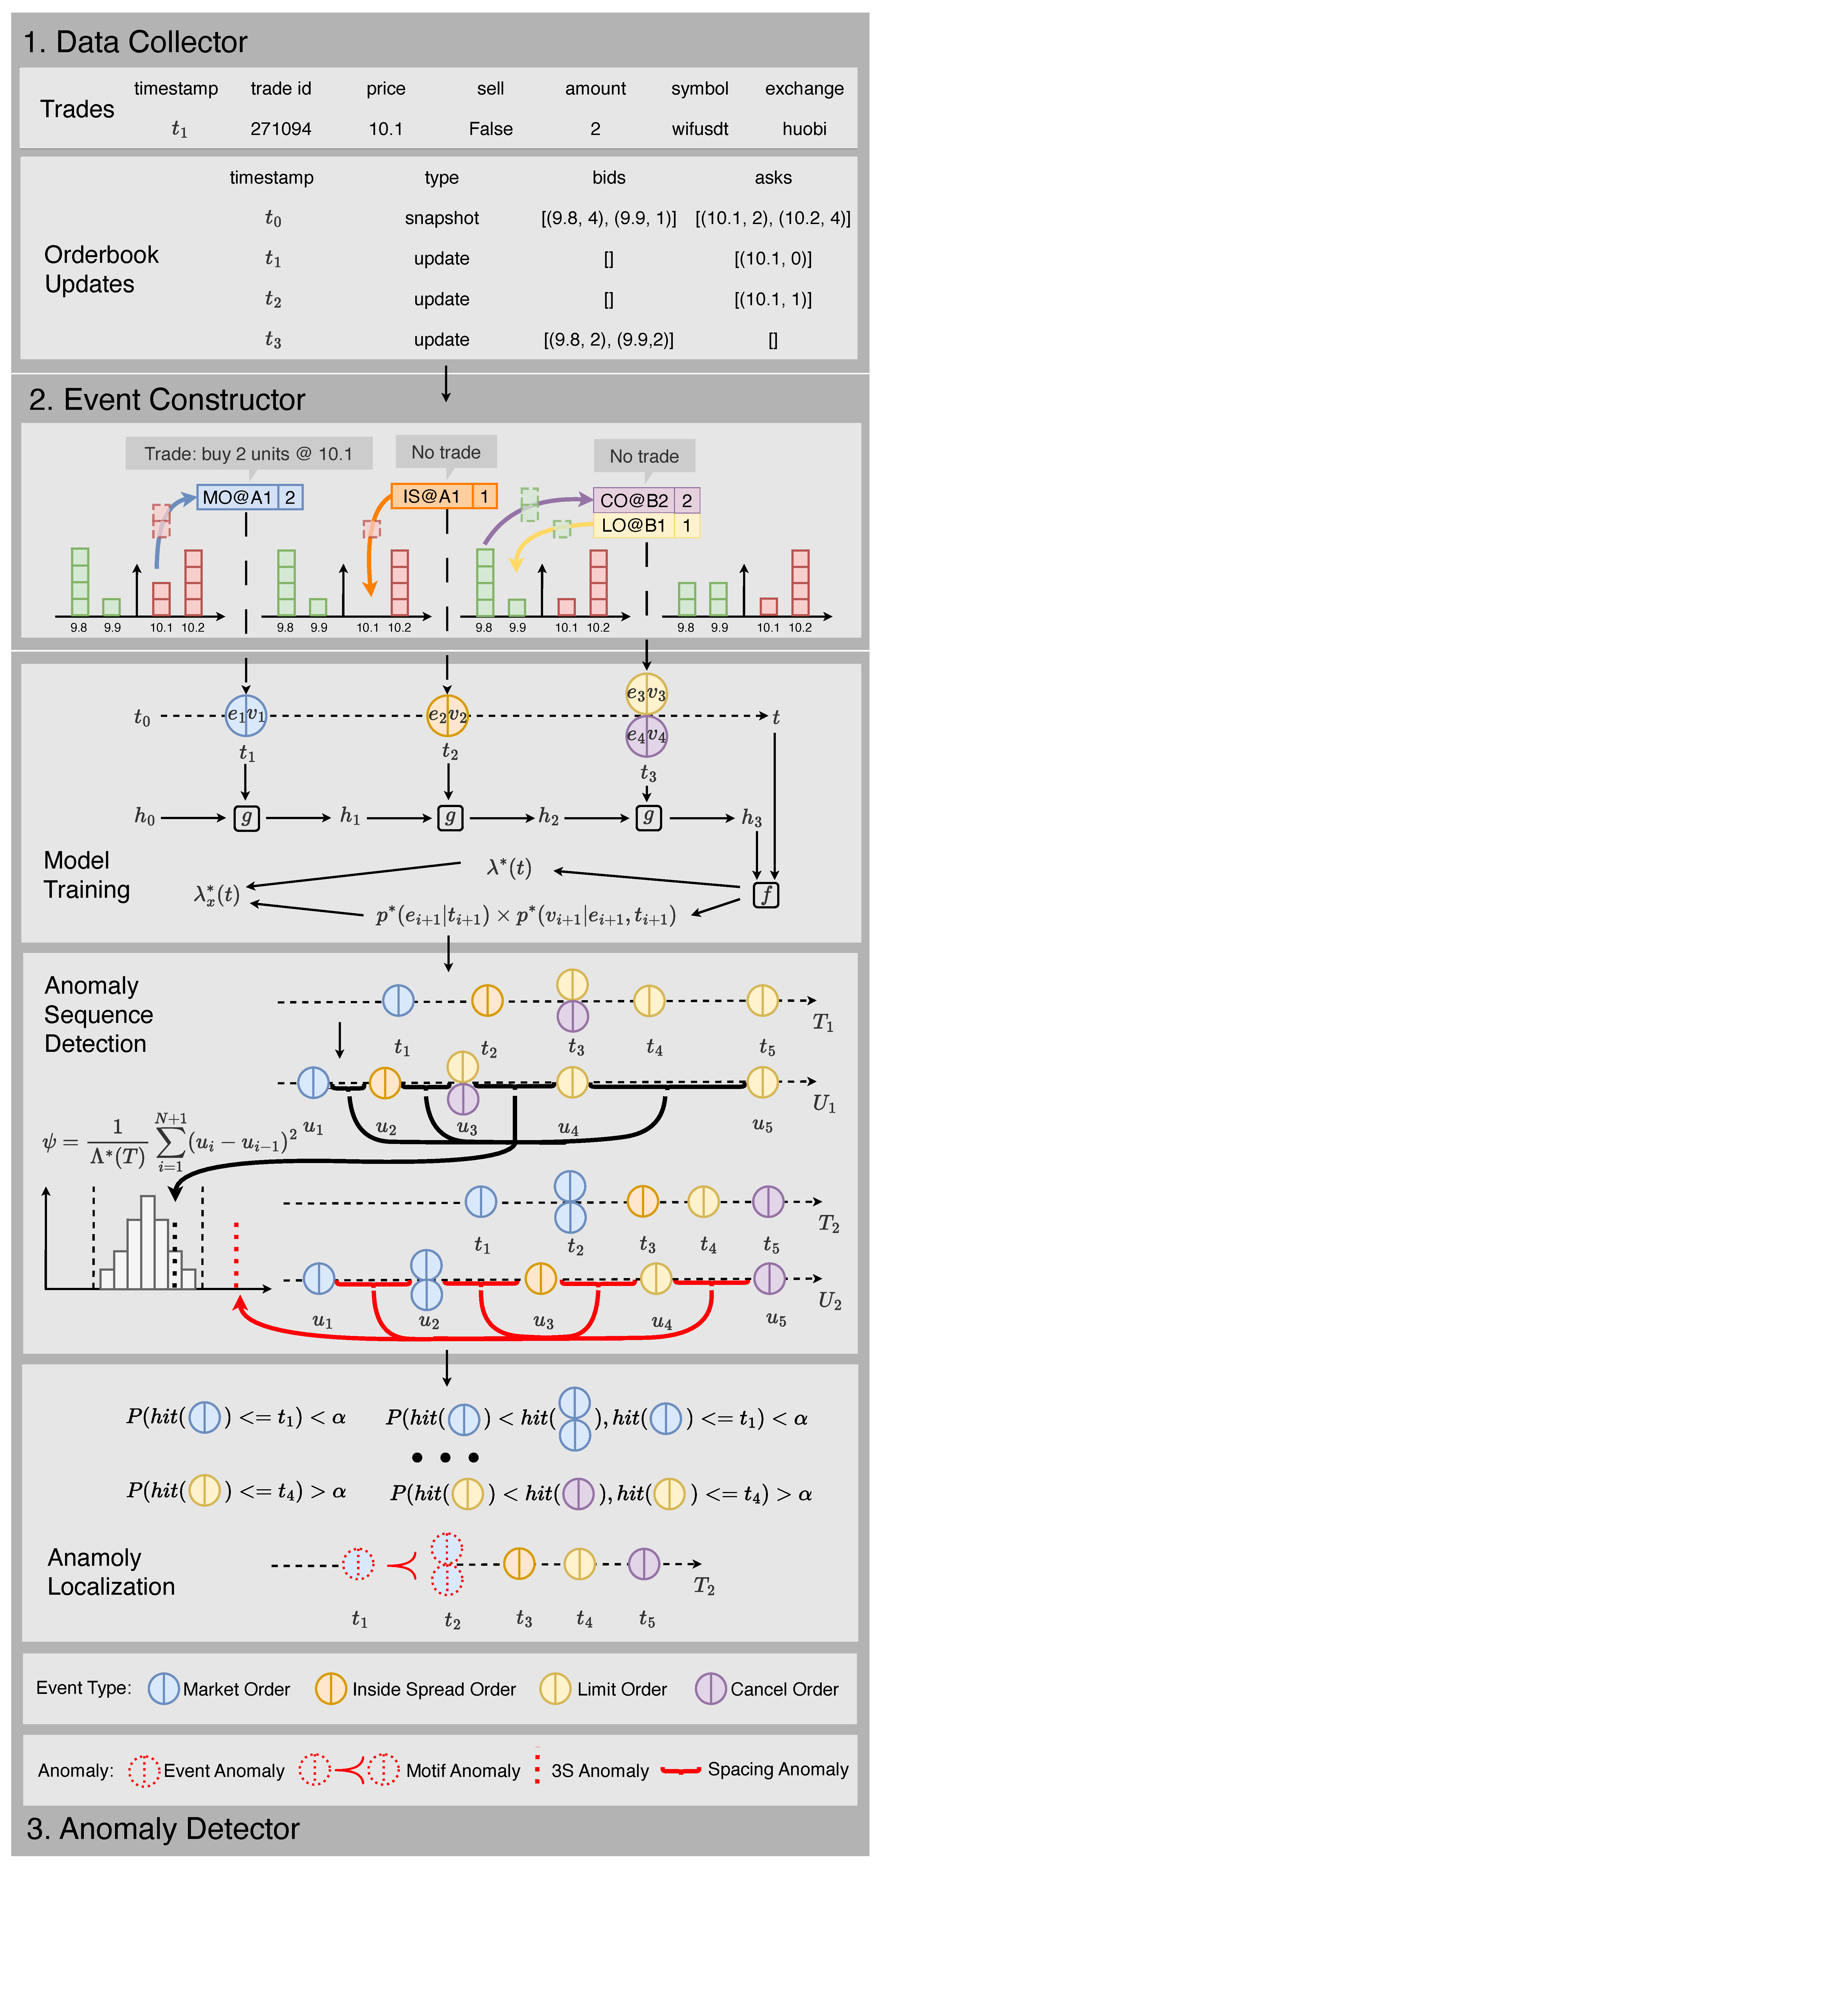
\includegraphics[width=0.6\linewidth]{img/tfow_pipeline.pdf}
  % \caption{Pipeline consists of three modules: (i) data collector: that gathers trades and order book updates; (ii) an event constructor: that transforms raw updates and trades into sequential sets of order events; and (iii) an anomaly detector, trained on large-scale data, which scores motif-filtered event sequences for abnormal patterns.  }
    \caption{\ac{tfow} consists of three modules: (i) data collector; (ii) Event constructor; and (iii) anomaly detector. Note, (a, b) here is not an event but the actual price and depth.}
  \label{fig:pipeline}
\end{figure} 
\FloatBarrier




\subsection{Data Collector}
We obtain both trade and Level-2 limit order book data from Kaiko~\cite{Kaiko2025TheKaiko}, a leading institutional provider of digital asset market data. In partnership with Cloudburst Technologies~\cite{Cloudburst2025CloudburstTechnologies}, a leading firm specializing in detecting and mitigating market manipulation, we establish the data collector. Level-2 limit order book updates are continuously streamed to a Google Cloud Storage bucket, providing full-depth market coverage. Each update record contains precise timestamps, update types (snapshots or liquidity updates), and the corresponding price–volume information for bid and ask levels. Complementary trade data are retrieved via Kaiko’s API and temporally aligned with the order book stream, enabling synchronized analysis of trading activity and order flow dynamics.




\subsection{Event constructor}
\label{subsec:event-construction}
\begin{figure}[!h]
  \centering  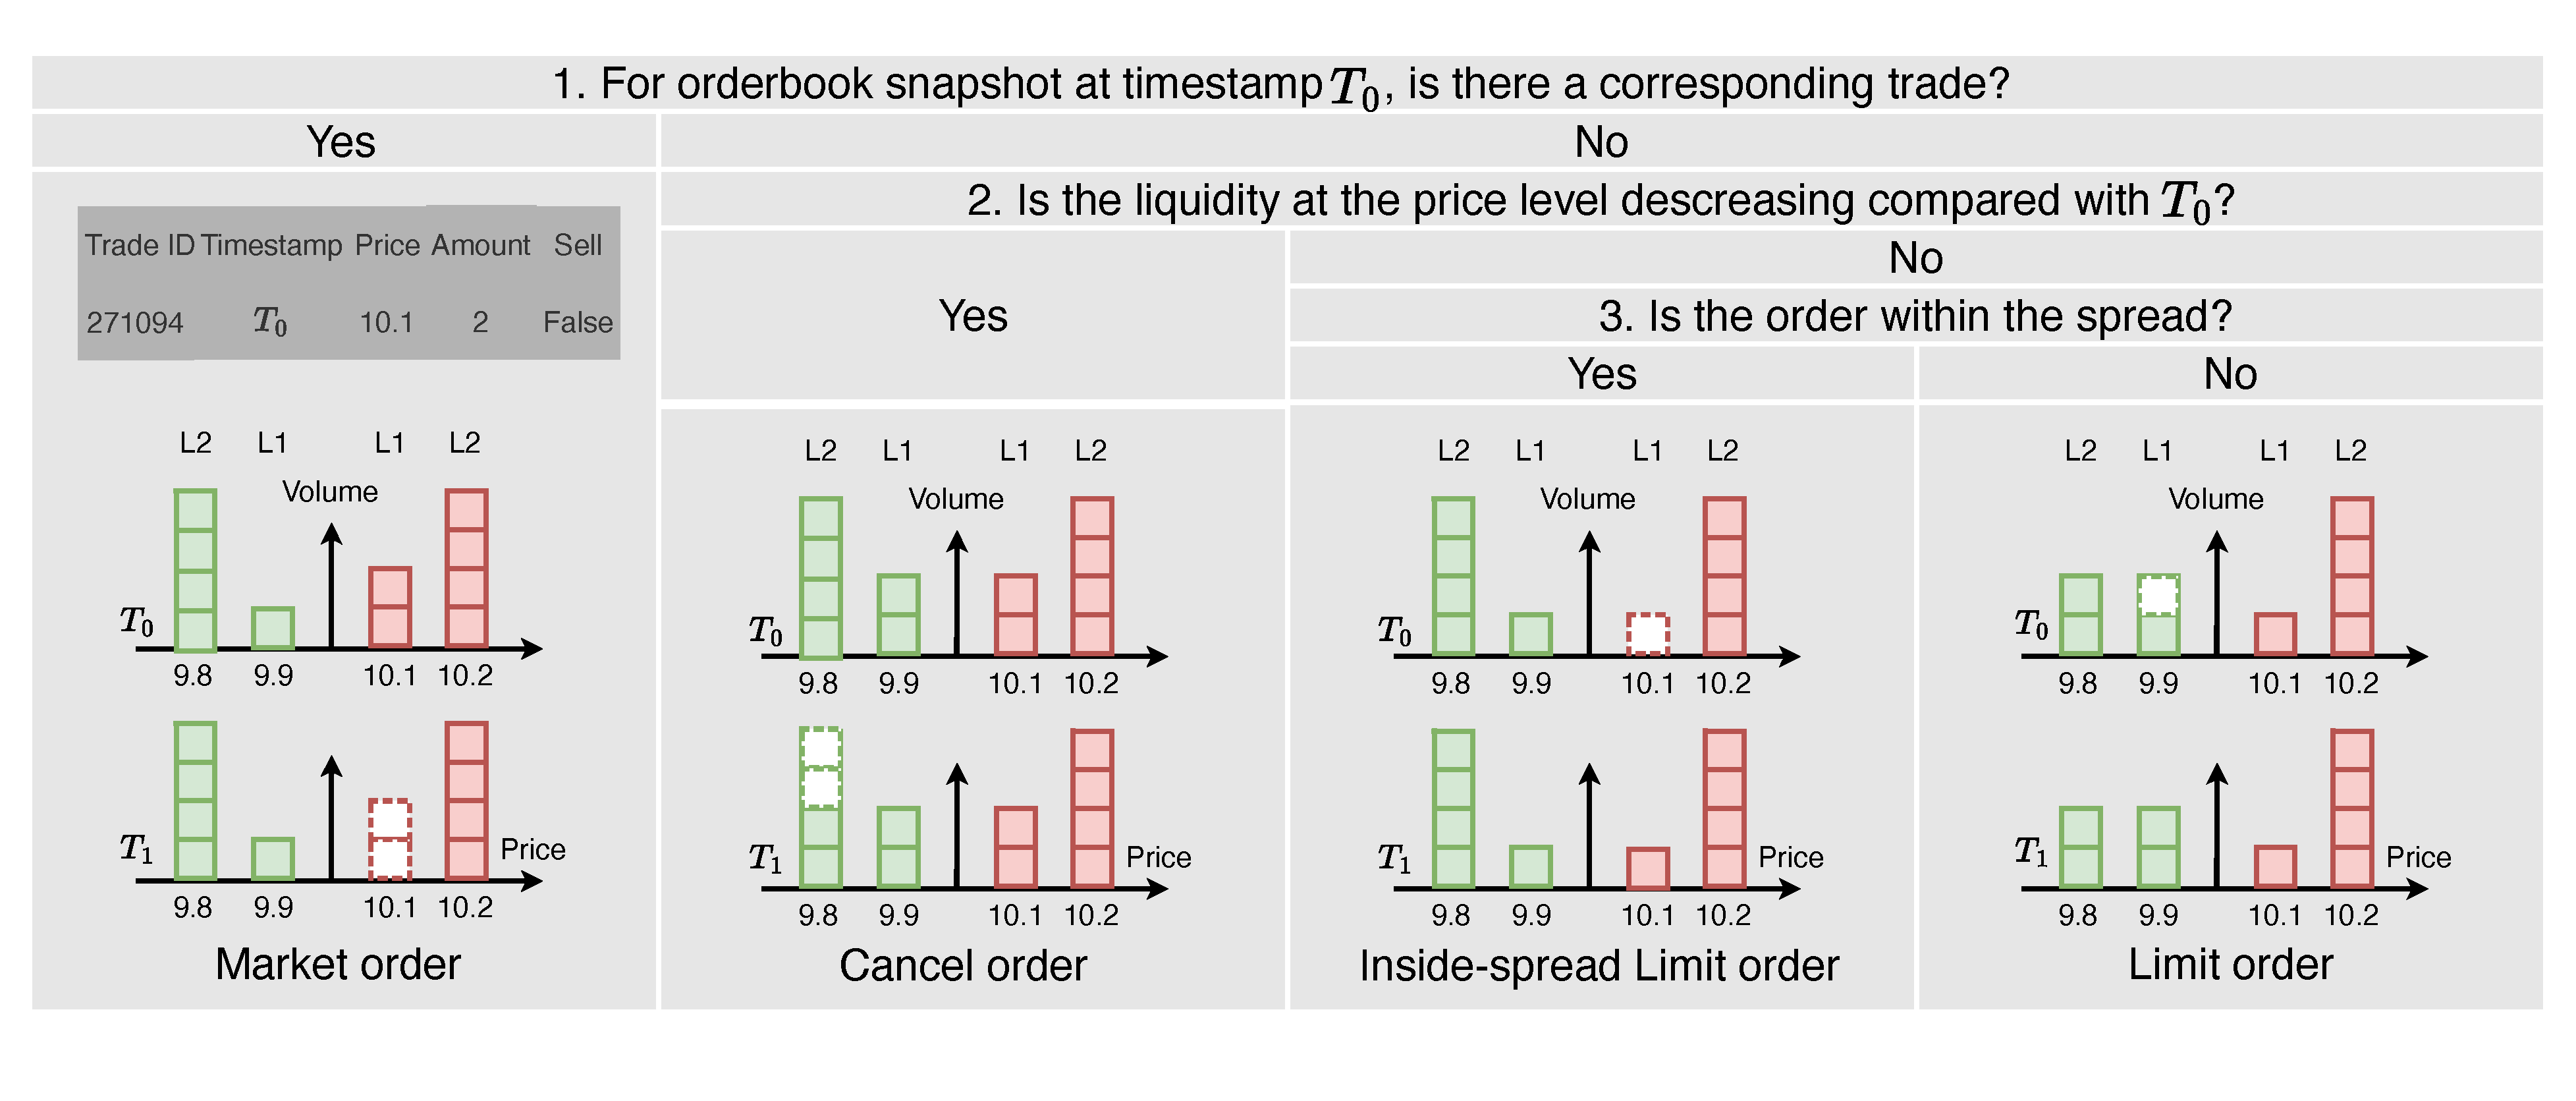
\includegraphics[width=\linewidth]{img/event_construction.pdf}
  \caption{Event construction for 4 order types through 3 questions. Each question is a decision tree for classification. We start with question 1 to question 3. Note, market order is a case of liquidity decreasing.}
  \label{fig:graph_infer}
\end{figure} 
\FloatBarrier



To apply point process modeling to high-frequency limit order book (LOB) data, we represent market dynamics as a sequence of \textbf{event sets}. We consider the top $K=10$ levels on each side (bid and ask).  

\paragraph{Atomic Events.}  
We define a finite set $E$ of \emph{atomic event types}, each denoted $e=(c,s,\delta)$, where:
\begin{itemize}[leftmargin=1.2em]
    \item $c \in \{\text{LO}, \text{MO}, \text{CO}, \text{IS}\}$ is the \emph{event class}:
        \begin{itemize}
            \item \textbf{Limit Order (LO)}: liquidity provision at one of the top-$K$ levels.
            \item \textbf{Cancel Order (CO)}: liquidity withdrawal at one of the top-$K$ levels.
            \item \textbf{Market Order (MO)}: liquidity consumption at the best quote.
            \item \textbf{Inside-Spread Order (IS)}: a new order placed inside the spread, improving the prevailing best quote.
        \end{itemize}
    \item $s \in \{b,a\}$ is the \emph{side} (bid or ask).
    \item $\delta$ is the \emph{level index}:
        \begin{itemize}
            \item For LO/CO, $\delta \in \{1,\dots,K\}$ indicates distance from the best quote ($\delta=1$ = best bid/ask, $\delta=10$ = tenth level).
            \item For MO, $\delta=1$ always, since market orders execute against the current best quote.
            \item For IS, $\delta \in \{1,\dots,K\}$ denotes the number of ticks by which the new quote improves the spread (e.g., $\text{IS}_{b,2}$ = new bid order two ticks inside the spread).
        \end{itemize}
\end{itemize}

\paragraph{Event Construction from LOB and Trade Data.}  
As illustrated in \autoref{fig:graph_infer}, each atomic order event is inferred by differencing consecutive Level-2 order book snapshots and aligning them with trade records at identical timestamps. Because trades and book updates are perfectly synchronized in both time and volume, every observed change can be classified without ambiguity through a three-step decision tree.
First, if the best-quote liquidity decreases and a trade is recorded at the same price, the change corresponds to a \textbf{Market Order}—a direct execution against standing quotes.
Second, if liquidity decreases at any level without a matching trade, the reduction represents a \textbf{Cancel Order}, reflecting liquidity withdrawal.
Finally, when liquidity increases, the classification depends on the price position: if the new order appears inside the spread, it forms an \textbf{Inside-Spread Order}; otherwise, it is a \textbf{Limit Order} placed within the existing book depth. This rule set ensures exhaustive mapping from raw order book and trade data into atomic order events, enabling a consistent foundation for downstream temporal modeling and anomaly detection.





\paragraph{Event Sets.} 
In crypto limit order books, each event is associated with a set of items. In other words, multiple atomic events may occur simultaneously at the same timestamp. We therefore allow \emph{event sets} at each time $t_i$:
\[
X_{t_i} = \{(e_{i_1}, v(e_{i_1})), \dots, (e_{i_n}, v(e_{i_n}))\},
\]
where $e_{i_n} \in \mathcal{E}$ are atomic events and $v(e_{i_n})$ their volume marks.

\subsection{State-Dependent Set-MTPP Backbone}

\paragraph{Intuition.}
The event flow of a limit order book is governed not only by past order-flow history, but also by the contemporaneous market condition. In particular, the relative dominance of bid-side and ask-side queues affects the likelihood of future submissions, cancellations, executions, and inside-spread improvements. Following the state-dependent neural Hawkes formulation of Shi and Cartlidge, we incorporate a discrete market state into the intensity model so that TFOW captures both temporal dependence and the current order-book regime. Unlike Shi and Cartlidge, however, we do \emph{not} adopt the parallel CT-LSTM architecture. We only use their state mechanism and retain a single continuous-time neural backbone, which is more suitable for our set-valued marked event representation and keeps the model compact.

\paragraph{Market state.}
Let \(v_b^{(1)}(t)\) and \(v_a^{(1)}(t)\) denote the top-of-book bid and ask queue volumes at time \(t\). We define the queue-imbalance indicator
\[
I(t)=\frac{v_b^{(1)}(t)-v_a^{(1)}(t)}{v_b^{(1)}(t)+v_a^{(1)}(t)}.
\]
Given a threshold \(\theta \in (0,1)\), we discretize the market state as
\[
s_t=
\begin{cases}
0, & I(t)\in[-1,-\theta),\\[2mm]
1, & I(t)\in[-\theta,\theta],\\[2mm]
2, & I(t)\in(\theta,1].
\end{cases}
\]
These three regimes correspond to ask-dominant, balanced, and bid-dominant markets, respectively.

\paragraph{State-dependent hidden dynamics.}
Let \(\mathcal H_t\) denote the history of all event sets and volume marks up to time \(t\). As defined in Section 4.2, each timestamp \(t_i\) is associated with an event set
\[
X_{t_i}=\{(e_{i1},v(e_{i1})),\dots,(e_{in_i},v(e_{in_i}))\},
\]
where \(e_{im}\in \mathcal{E} \) is an atomic event and \(v(e_{im})\) is its volume mark. TFOW encodes the sequence of past event sets together with the current market state into a continuous-time hidden representation \(h_t\). Between event times, the hidden state decays continuously; at each event time, it is updated using the newly observed event set and the contemporaneous state. This follows the state-dependent neural point process principle that the intensity is decoded from a latent state rather than specified by an additive Hawkes kernel.

We define the baseline intensity by
\[
\lambda_{\theta}^{\mathrm{base}}(t \mid \mathcal H_t, s_t)
=
f_{\theta}(h_t,s_t),
\]
where \(f_{\theta}(\cdot)\) is a positive decoder. In practice, \(f_{\theta}\) may be implemented using a softplus output layer to ensure non-negativity of the intensity.

\paragraph{State transition.}
The market state is allowed to evolve jointly with the event process. Following Shi and Cartlidge, after the event set at time \(t_i\) is observed, the next state is governed by an event-conditioned transition distribution
\[
P(s_{t_i}\mid \mathcal H_{t_i^-}, y_i, s_{t_i^-}) \sim \phi_{y_i,s_{t_i^-}},
\]
where \(y_i\) is the event-type summary associated with timestamp \(t_i\), and \(\phi\in\mathbb R^{K\times W\times W}\) is a discrete transition tensor. In our implementation, \(\phi\) is estimated offline via empirical transition counting, separately from the neural network parameters.

\paragraph{Compensator.}
The compensator associated with the baseline state-dependent intensity is
\[
\Lambda_{\theta}^{\mathrm{base}}(t)
=
\int_0^t \lambda_{\theta}^{\mathrm{base}}(u\mid \mathcal H_u,s_u)\,du.
\]
This baseline Set-MTPP models the structural dynamics of normal order flow. The next subsection introduces a second-order diagnostic derived from compensator increments and uses it to adapt the baseline intensity online.


\subsection{Differential 3S as a Second-Order Diagnostic}

\paragraph{Intuition.}
A correctly specified temporal point process becomes a unit-rate Poisson process after the random time change induced by its compensator. Therefore, on the transformed clock, the inter-event gaps should behave like i.i.d.\ \(\mathrm{Exp}(1)\) random variables. This implies not only that the model gets the expected event count right, but also that it gets the geometry of event spacing right. In particular, if \(\Delta u_i \sim \mathrm{Exp}(1)\), then
\[
\mathbb E[\Delta u_i]=1,
\qquad
\mathrm{Var}(\Delta u_i)=1,
\qquad
\mathbb E[(\Delta u_i)^2]=2.
\]
The original 3S statistic is built from squared transformed gaps and therefore probes this second-moment structure. Intuitively, first-order residuals ask whether the model gets the \emph{number of arrivals} right, while squared compensator increments ask whether it gets the \emph{irregularity of event timing} right. This motivates a sequential second-order diagnostic for TFOW.

\paragraph{Compensator increments.}
Let
\[
u_i=\Lambda_{\theta}^{\mathrm{base}}(t_i),
\qquad
\Delta u_i=u_i-u_{i-1}
=
\int_{t_{i-1}}^{t_i}\lambda_{\theta}^{\mathrm{base}}(u\mid \mathcal H_u,s_u)\,du.
\]
If the baseline state-dependent model is correctly specified, then by the random time-change theorem,
\[
\Delta u_i \overset{i.i.d.}{\sim} \mathrm{Exp}(1).
\]
Hence,
\[
\mathbb E[(\Delta u_i)^2]=2.
\]
This second moment is the key quantity behind 3S. Rather than computing a global goodness-of-fit statistic over an entire transformed sequence, we extract an event-level residual from the same quadratic intuition.

\paragraph{Differential 3S residual.}
We define the differential 3S residual by
\[
r_i^{(2)}=(\Delta u_i)^2-2.
\]
Under the correctly specified model,
\[
\mathbb E[r_i^{(2)}]=0.
\]
Thus, \(r_i^{(2)}\) measures the local second-order deviation of transformed spacing from the Poisson benchmark. Positive values indicate abnormally irregular, bursty, or dispersed spacing on the compensator clock, whereas negative values indicate overly regular spacing. In this sense, \(r_i^{(2)}\) is a quadratic second-order diagnostic on compensator increments.

\paragraph{Smoothed deviation state.}
To obtain a stable sequential signal, we smooth the event-level residual recursively:
\[
d_i^{(2)}
=
\rho d_{i-1}^{(2)}+(1-\rho)r_i^{(2)},
\qquad \rho\in[0,1).
\]
The process \(d_i^{(2)}\) summarizes recent second-order deviations in transformed event spacing. Unlike a rolling-window goodness-of-fit test, this construction is incremental and naturally compatible with sequential modeling.

\paragraph{Deviation-controlled intensity.}
We incorporate the second-order deviation signal into TFOW through a multiplicative correction of the baseline state-dependent intensity:
\[
\lambda_{\theta}(t\mid \mathcal H_t,s_t)
=
\lambda_{\theta}^{\mathrm{base}}(t\mid \mathcal H_t,s_t)
\exp\!\big(\beta d_i^{(2)}\big),
\qquad t\in(t_i,t_{i+1}],
\]
where \(\beta\in\mathbb R\) is learnable. Equivalently,
\[
\log \lambda_{\theta}(t\mid \mathcal H_t,s_t)
=
\log \lambda_{\theta}^{\mathrm{base}}(t\mid \mathcal H_t,s_t)
+
\beta d_i^{(2)}.
\]
This decomposition separates structural order-flow dynamics from second-order temporal irregularity: the baseline term captures the dynamics explained by event history and imbalance state, while the differential 3S term captures residual spacing abnormalities not explained by the structural model.

\paragraph{Discussion.}
The proposed diagnostic is complementary to first-order residual monitoring. Standard martingale residuals compare realized and expected counts and are therefore sensitive to count drift. In contrast, differential 3S probes the second moment of transformed waiting times and is sensitive to clustering, dispersion, and abnormal spacing geometry. In crypto limit order books, this allows TFOW to respond not only to unusual event volume, but also to strategically timed bursts, pauses, and irregular cancellation or inside-spread patterns that are characteristic of manipulative flow.


\subsection{Differential 3S as a Second-Order Diagnostic on Compensator Increments}



\subsubsection{State-Dependent Intensity Modeling}

In limit order book markets, the arrival of events is influenced not only by past order flow but also by the contemporaneous market condition. Recent work therefore extends neural Hawkes processes by conditioning the event intensity on a discrete market state that summarizes the current order book configuration~\cite{Shi2022StateSimulation}. 

Formally, let $H_t$ denote the event history and $s_t$ a state variable derived from the order book. The conditional intensity for event type $k$ is then modeled as
\begin{equation}
\lambda_k(t \mid H_t, s_t) = f_k(h_t, s_t),
\end{equation}
where $h_t$ is a latent representation of past events produced by a continuous-time recurrent mechanism and $f_k(\cdot)$ decodes the instantaneous arrival rate. The state variable typically partitions the market into regimes such as bid-dominant, balanced, or ask-dominant based on queue imbalance.


% \subsection{Deviation-Controlled Intensity and Dual-Deviation Decomposition}
% \label{subsec:deviation_controlled}

We extend the intensity formulation by introducing a deviation-controlled feedback mechanism that enables explicit separation between structural dynamics and market-driven temporal irregularity.

\paragraph{Baseline TFOW intensity.}
Model's conditional intensity is
%
\begin{equation}
\lambda_0(t)
=
\lambda(h_t, x_t),
\label{eq:tfow_baseline_intensity2}
\end{equation}
%
where $h_t$ encodes historical order flow and $x_t$ denotes the imbalance regime state. The associated compensator is
%
\begin{equation}
\Lambda_0(t)
=
\int_0^t \lambda_0(\tau)\, d\tau.
\label{eq:tfow_compensator2}
\end{equation}
%
The derivation of $\lambda_0(t)$ and $\Lambda_0(t)$ follows the temporal point process.

%
\begin{equation}
\Delta u_i
=
\Lambda(t_i) - \Lambda(t_{i-1})
=
\int_{t_{i-1}}^{t_i} \lambda(\tau)\, d\tau.
\label{eq:delta_u2}
\end{equation}
%
Under correct model specification, the time-rescaling theorem implies
%
\[
\Delta u_i \sim \text{Exp}(1),
\]
%
i.e., rescaled inter-arrival times are i.i.d. exponential with unit mean.




\paragraph{Intuition.}
A correctly specified temporal point process should become a unit-rate Poisson process after the random time change induced by its compensator. On this transformed clock, the inter-event gaps should behave like i.i.d.\ $\mathrm{Exp}(1)$ variables. This implies not only a correct \emph{first-order} behavior, i.e., the expected number of arrivals matches the compensator, but also a correct \emph{second-order} behavior, i.e., the transformed waiting times have the right dispersion and spacing geometry. In particular, if $\Delta u_i \sim \mathrm{Exp}(1)$, then
\[
\mathbb{E}[\Delta u_i]=1,
\qquad
\mathrm{Var}(\Delta u_i)=1,
\qquad
\mathbb{E}[(\Delta u_i)^2]=2.
\]
The classical 3S statistic is built from squared transformed gaps and therefore probes this second-moment structure. Intuitively, while first-order residuals measure whether the model gets the \emph{event count} right, squared compensator increments measure whether the model gets the \emph{timing irregularity} right. Large values indicate abnormally bursty or dispersed spacing on the transformed clock, while small values indicate overly regular spacing. This makes the second moment of compensator increments a natural second-order diagnostic for local model misspecification.

Formally, let $\lambda_\theta(t \mid \mathcal{H}_t)$ denote the conditional intensity produced by TFOW, and define its compensator
\[
\Lambda_\theta(t)=\int_0^t \lambda_\theta(u \mid \mathcal{H}_u)\,du.
\]
For the observed event times $\{t_i\}_{i=1}^N$, define the transformed times
\[
u_i=\Lambda_\theta(t_i),
\qquad
\Delta u_i=u_i-u_{i-1}.
\]
By the random time-change theorem, if the model is correctly specified, then the transformed process is a standard Poisson process and the increments satisfy
\[
\Delta u_i \overset{i.i.d.}{\sim} \mathrm{Exp}(1).
\]

Motivated by the quadratic structure of 3S, we define the event-level \emph{differential 3S residual}
\[
r_i^{(2)} = (\Delta u_i)^2 - 2.
\]
Since $\mathbb{E}[(\Delta u_i)^2]=2$ under the Poisson null, $r_i^{(2)}$ is centered:
\[
\mathbb{E}[r_i^{(2)}]=0.
\]
Thus, $r_i^{(2)}$ quantifies the local second-order deviation of the transformed spacing from the model-implied $\mathrm{Exp}(1)$ benchmark. Specifically, $r_i^{(2)}>0$ indicates abnormally irregular transformed spacing, whereas $r_i^{(2)}<0$ indicates overly regular spacing.

To obtain a stable sequential signal, we smooth the event-level residual recursively:
\[
d_i^{(2)} = \rho d_{i-1}^{(2)} + (1-\rho) r_i^{(2)},
\qquad \rho \in [0,1).
\]
The state $d_i^{(2)}$ summarizes recent second-order deviations on the compensator clock. We then incorporate it into the conditional intensity as a multiplicative correction:
\[
\lambda_\theta(t \mid \mathcal{H}_t)
=
\lambda_\theta^{\mathrm{base}}(t \mid \mathcal{H}_t)
\exp\!\big(\beta d_i^{(2)}\big),
\qquad t \in (t_i, t_{i+1}],
\]
where $\lambda_\theta^{\mathrm{base}}$ is the base TFOW intensity and $\beta$ controls the sensitivity to second-order deviation.

This construction is closely related in spirit to 3S, since both are driven by squared transformed inter-event gaps. The distinction is that the original 3S statistic is a \emph{global} goodness-of-fit functional, whereas our formulation extracts an \emph{incremental} second-order residual process suitable for sequential modeling. Consequently, TFOW is able to respond online not only to the structural order-flow state, but also to recent deviations in the timing geometry of events relative to the compensator-implied Poisson benchmark.

\paragraph{Discussion.}
The proposed diagnostic is complementary to first-order residual monitoring. Standard martingale residuals compare observed and expected counts through $N(t)-\Lambda_\theta(t)$, and are therefore sensitive to count drift. In contrast, $r_i^{(2)}$ probes the second moment of transformed waiting times and is sensitive to local irregularity in event spacing. In microstructure settings, this allows the model to detect regime shifts that manifest not only through excess event volume, but also through abnormal clustering, dispersion, or regularization of order-flow timing.

% \subsection{Differential 3S as a Second-Order Residual}

% \paragraph{Intuition.}
% After compensator-based time rescaling, a correctly specified point process should become a unit-rate Poisson process. Hence the transformed inter-event gaps should satisfy $\Delta u_i \overset{i.i.d.}{\sim}\mathrm{Exp}(1)$, implying
% \[
% \mathbb{E}[\Delta u_i]=1,
% \qquad
% \mathbb{E}[(\Delta u_i)^2]=2.
% \]
% The first quantity controls average arrival rate, while the second controls spacing irregularity. Therefore, if first-order residuals measure whether the model gets the event count right, squared transformed gaps measure whether the model gets the timing geometry right. This observation motivates a second-order diagnostic derived from the 3S principle.

% Let
% \[
% \Lambda_\theta(t)=\int_0^t \lambda_\theta(u \mid \mathcal{H}_u)\,du,
% \qquad
% u_i=\Lambda_\theta(t_i),
% \qquad
% \Delta u_i=u_i-u_{i-1}.
% \]
% Under correct specification, $\Delta u_i \overset{i.i.d.}{\sim}\mathrm{Exp}(1)$. We therefore define the differential 3S residual
% \[
% r_i^{(2)}=(\Delta u_i)^2-2,
% \]
% which satisfies $\mathbb{E}[r_i^{(2)}]=0$ under the null. Positive values indicate abnormally irregular transformed spacing, while negative values indicate overly regular spacing.

% To stabilize this event-level signal, we define
% \[
% d_i^{(2)}=\rho d_{i-1}^{(2)}+(1-\rho)r_i^{(2)},
% \qquad \rho\in[0,1),
% \]
% and use it to modulate the base TFOW intensity:
% \[
% \lambda_\theta(t \mid \mathcal{H}_t)
% =
% \lambda_\theta^{\mathrm{base}}(t \mid \mathcal{H}_t)
% \exp(\beta d_i^{(2)}),
% \qquad t\in(t_i,t_{i+1}].
% \]
% Unlike the original 3S statistic, which is a global goodness-of-fit functional over a transformed sequence, our formulation yields a sequential second-order residual process. This allows TFOW to adapt online to recent deviations in the local spacing structure of order-flow events on the compensator clock.


\subsection{State-Dependent Intensity with Deviation Feedback}



\paragraph{Deviation-controlled intensity.}
We define the modified intensity:
%
\begin{equation}
\boxed{
\lambda(t)
=
\lambda_0(t)
\cdot
\exp(\beta s_t),
}
\label{eq:deviation_controlled_lambda2}
\end{equation}
%
with $\beta \in \mathbb{R}$ learnable.

Taking logarithms,
%
\begin{equation}
\log \lambda(t)
=
\log \lambda_0(t)
+
\beta s_t.
\label{eq:log_decomposition2}
\end{equation}


The baseline term $\lambda_0(t)$ captures structural dynamics encoded in $(h_t, x_t)$, which summarize event history and regime information. Any deviation in arrival behavior not explained by these structural components must manifest through systematic distortions of rescaled-time spacings.

Since $s_t$ is computed solely from compensator increments $\{\Delta u_i\}$, it measures inconsistency between predicted and realized temporal spacing. Importantly, $s_t$ depends only on the temporal arrangement of events relative to the model's own predicted intensity and under correct structural modeling, fluctuations in $s_t$ arise from genuine clustering or dispersion in the market. Persistent elevation of $s_t$ corresponds to bursty arrivals (volatility shocks, liquidation cascades), and suppressed $s_t$ corresponds to under-dispersed flow (liquidity drought, inactivity).

Therefore, $\beta s_t$ quantifies multiplicative amplification (or attenuation) of structural intensity required to reconcile predicted flow with observed temporal irregularity.

In other words,
%
\begin{equation}
\beta s_t
=
\log \frac{\lambda(t)}{\lambda_0(t)},
\end{equation}
%
which measures the deviation of realized market activity from structurally expected activity.


Let $\hat{\lambda}_{\text{obs}}(t)$ denote empirical intensity estimated over a short window. We define

\begin{align}
D_{\text{market}}(t)
&=
\beta s_t,
\\
D_{\text{model}}(t)
&=
\left|
\log \hat{\lambda}_{\text{obs}}(t)
-
\log \lambda(t)
\right|.
\end{align}

Then
%
\begin{equation}
\log \hat{\lambda}_{\text{obs}}(t)
=
\log \lambda_0(t)
+
D_{\text{market}}(t)
+
\epsilon_t,
\end{equation}
%
where $\epsilon_t$ corresponds to residual model misspecification.

\paragraph{Interpretational summary.}

\begin{itemize}
\item $\lambda_0(t)$: structural prediction from TFOW history and regime.
\item $\beta s_t$: systematic temporal irregularity induced by market dynamics.
\item $\epsilon_t$: unexplained residual error.
\end{itemize}

Thus, $\beta s_t$ represents market-driven deviation because it quantifies the multiplicative adjustment necessary to align structural intensity with empirically observed clustering, independently of latent state encoding.

This decomposition renders temporal abnormality identifiable and enables real-time attribution of intensity variation to market shocks rather than model error.

% This formulation introduces an event–state interaction: the current state influences the probability of future events, while newly arriving events update the market state. Such state-dependent point processes provide a flexible way to capture the coupling between order flow dynamics and the evolving order book environment~\cite{shi2022state}.

% We model the order flow as a marked temporal point process with conditional
% intensity depending on both the event history and the latent market state.
% Let $\mathcal{H}_t = \{(t_i, m_i)\}_{t_i < t}$ denote the event history,
% where $t_i$ is the event time and $m_i$ is the event mark
% (e.g., event type, side, level, and volume).
% A neural encoder (e.g., CT-LSTM or Transformer) maps the history to a hidden state

% \begin{equation}
% h_t = \mathrm{Enc}(\mathcal{H}_t).
% \end{equation}

% To capture regime-dependent market dynamics, we introduce a latent market
% state $z_t \in \Delta^{K-1}$, where $\Delta^{K-1}$ denotes the probability
% simplex over $K$ regimes.
% The regime posterior is inferred from the hidden state

% \begin{equation}
% z_t = \mathrm{softmax}(W_z h_t).
% \end{equation}

% The structural baseline intensity is then defined as a mixture of
% regime-specific intensities

% \begin{equation}
% \lambda_0(t \mid \mathcal{H}_t, z_t)
% =
% \sum_{k=1}^{K}
% z_{t,k}\,
% \lambda_k(h_t),
% \end{equation}

% where $\lambda_k(\cdot)$ denotes the intensity associated with regime $k$.

% \paragraph{Deviation Feedback via Rolling 3S.}
% While $\lambda_0(t)$ captures the structural dynamics implied by the model,
% real markets frequently exhibit bursty or irregular arrival patterns that
% cannot be fully explained by the baseline intensity.
% To capture such deviations online, we introduce a rolling deviation statistic
% based on the squared spacings of the time-rescaled process.

% Let $\Lambda(t) = \int_0^t \lambda_0(\tau) d\tau$ denote the compensator of
% the baseline model.
% For events $t_i$ in a rolling window $(t-W,t)$, we define the rescaled spacings

% \begin{equation}
% \Delta u_i = \Lambda(t_i) - \Lambda(t_{i-1}),
% \end{equation}

% and the rolling deviation statistic

% \begin{equation}
% s_t
% =
% \frac{1}{\Lambda(t) - \Lambda(t-W)}
% \sum_{t_i \in (t-W,t)}
% (\Delta u_i)^2 .
% \end{equation}

% Under correct model specification, the rescaled spacings follow the exponential
% distribution implied by the time-rescaling theorem, and $s_t$ remains stable.
% Large values of $s_t$ therefore indicate bursty or irregular order flow.

% \paragraph{Deviation-Controlled Intensity.}
% We incorporate this deviation signal directly into the intensity via a
% multiplicative feedback mechanism

% \begin{equation}
% \lambda(t)
% =
% \lambda_0(t \mid \mathcal{H}_t, z_t)
% \cdot
% \exp(\beta s_t),
% \end{equation}

% where $\beta$ is a learnable parameter controlling the sensitivity of the
% intensity to market deviations.
% This formulation yields a state-dependent intensity that adapts in real time
% to deviations in the observed order flow.

% \paragraph{Training Objective.}
% The model is trained via maximum likelihood of the marked point process

% \begin{equation}
% \mathcal{L}
% =
% \sum_i \log \lambda(t_i)
% -
% \int_0^T \lambda(t) dt .
% \end{equation}

% By jointly learning the baseline intensity $\lambda_0(t)$,
% the regime state $z_t$, and the deviation feedback coefficient $\beta$,
% the model captures both the structural dynamics of the order flow
% and transient deviations from the learned equilibrium dynamics.

\subsubsection{Model Training}

!!!* train baseline intensity first
* compute differential 3S from detached compensator increments
* feed it back as a correction feature

\paragraph{Modeling Event Type and Volume in Order book Data}

The event constructor outputs a sequence of set of events. Formally, let each event at time $t_i$ be represented as a tuple
\[
x_i = \big(e_i, v_i \big),
\]
where $e$ is the event type and $v_i \in \mathbb{R}^+$ is the corresponding volume. We factorize the conditional mark distribution as
\begin{equation}
p(x_i \mid t_i, H(t_i)) 
= p(e_i \mid t_i, H(t_i)) \cdot p(v_i \mid e_i, t_i, H(t_i)),
\label{eq:factorization}
\end{equation}
where $H(t_i)$ denotes the event history up to time $t_i$.  

\paragraph{Set-Valued Marked Temporal Point Processes (Set-MTPP)}
\label{subsec:set-mtpp}

Classical marked temporal point processes (MTPPs) assume that each event is associated with a single categorical mark. This simplification breaks down in crypto limit order book level-2 data nature, where multiple atomic events---such as simultaneous limit placements, cancellations, and executions---often occur at exactly the same timestamp. To properly capture these co-occurrences, we adopt the \emph{set-valued MTPP} framework \cite{Chang2023}, which generalizes neural MTPPs from singleton events to event \emph{sets}.

Formally, let the event history be
\[
H(T) = \{(\tau_i, X_i)\}_{i=1}^N,
\]
where $\tau_i \in \mathbb{R}^+$ is the $i$-th event time and $X_i \subseteq \{1,\dots,M\}$ is a finite subset of atomic event type $e$ . The history up to time $t$ is $H(t) = \{(\tau_j, X_j): \tau_j < t\}$.  

The process is parameterized by a ground intensity $\lambda^*(t)$ and a conditional distribution over sets $p^*(X \mid t,H(t))$. The marked intensity factorizes as
\[
\lambda^*_X(t) = \lambda^*(t)\,p^*(X \mid t, H(t)).
\]
Accordingly, the joint log-likelihood decomposes into temporal and set contributions:
\[
\mathcal{L}(H(T)) =
\underbrace{\sum_{i=1}^N \log \lambda^*(\tau_i) - \int_0^T \lambda^*(s)\,ds}_{\mathcal{L}_{\text{time}}}
+
\underbrace{\sum_{i=1}^N \log p^*(X_i \mid \tau_i, H(\tau_i))}_{\mathcal{L}_{\text{set}}}.
\]

Set-MTPPs therefore provide a principled generative framework for level-2 LOB modeling, separating the dynamics of \emph{when} events occur from \emph{which sets} of events occur. This enables likelihood-based inference over simultaneous market microstructural patterns.

\paragraph{Volume Set Multivariate Temporal Point Processes}
\label{subsec:vol-set-mtpp}

While set-MTPPs capture simultaneous event types, each LOB event also carries a continuous \emph{volume mark} that reflects liquidity provision or consumption. Volumes are heavy-tailed and constrained by available depth---features that categorical marks alone cannot capture. We therefore extend set-MTPPs to a \emph{volume-set-MTPP}, which models both the composition of event sets and their associated traded volumes under realistic market constraints.

At each event time $t_i$, we observe:
\[
X_i \subseteq \{1,\dots,M\}, \quad 
\mathbf{v}_{t_i} = \{v(e) \in \mathbb{R}_{>0} : e \in X_{t_i}\},
\]
where $X_{t_i}$ is the set of event types and $\mathbf{v}_{t_i}$ their associated volumes. The modeling task is to learn
\[
p(X_t, \mathbf{v}_t \mid H_t),
\]
where $H_t$ is the market history up to $t$.

\subparagraph{Set–Volume Factorization.}
We decouple set composition and volume magnitudes:
\[
p(X_t, \mathbf{v}_t \mid H_t) = p(X_t \mid H_t)\,\prod_{e \in X_t} p(v(e) \mid e, H_t, \text{cap}_t(e)).
\]
This allows the model to (i) capture co-occurrence structure in $p(X_t \mid H_t)$, (ii) model event-specific volume distributions, and (iii) respect market microstructure constraints via $\text{cap}_t(e)$.

\subparagraph{Dynamic Set Model.}
Event sets are modeled via conditionally independent Bernoulli variables:
\[
p(X_t=x \mid H_t) = \prod_{k=1}^K \rho_k(h_t)^{x_k}(1-\rho_k(h_t))^{1-x_k},
\]
with $\rho_k(h_t) = \sigma(w_k^\top n(h_t)+b_k)$ parameterized by the hidden state $h_t$.

% \subparagraph{Continuous Volume Modeling.}
% Volumes are drawn from truncated log-normal distributions:
% \[
% p(v \mid e,H_t,\text{cap}_t) = \frac{f_{\text{LN}}(v;\mu_e(h_t),\sigma_e(h_t))}{\Phi\!\left(\frac{\ln(\text{cap}_t)-\mu_e(h_t)}{\sigma_e(h_t)}\right)} \,\mathbbm{1}[0<v \leq \text{cap}_t],
% \]
% where $f_{\text{LN}}$ is the log-normal density and $\Phi$ the normal CDF. This avoids discretization artifacts and naturally incorporates capacity limits.

% \subparagraph{Market Constraints.}
% We encode order book feasibility as:
% \[
% \text{cap}_t(e)=
% \begin{cases}
% Q_{s,\ell}(t), & e \in \{\text{MO},\text{CO}\}_{s,\ell},\\
% \infty, & e \in \{\text{LO},\text{IS}\}_{s,\ell},
% \end{cases}
% \]
% where $Q_{s,\ell}(t)$ is the standing depth at side $s$, level $\ell$.

\subparagraph{Neural Architecture and Training.}
We employ a Neural Hawkes~\cite{Mei2017TheProcess} to produce hidden states $h_{d,t}$, with three prediction heads:
(i) an intensity head for timing $\lambda(t)$, 
(ii) a set head for $\{\rho_k(h_{d,t})\}$, and 
(iii) a volume head for $\{(\mu_k(h_{d,t}),\sigma_k(h_{d,t}))\}$.  
The loss decomposes as
\[
\mathcal{L} = \mathcal{L}_{\text{timing}} + \mathcal{L}_{\text{sets}} +  \,\mathcal{L}_{\text{volumes}},
\]
balancing temporal, set, and volume likelihood terms.

This formulation yields a principled and high-fidelity generative model of LOB microstructure—enabling both simulation and anomaly detection in high-frequency trading.


\subsection{Anomaly Detection}

Market manipulators deliberately inject crafted orders into otherwise normal order flows, perturbing the natural distribution of event timings, traded volumes, and directional dependencies between orders. Such distortions are inherently statistical and can therefore be detected through distributional tests on the reconstructed event history.

Formally, let the full observed history up to horizon $T$ be
\[
\mathcal{H}(T)
= \{(t_i, X_{t_i})\}_{i=1}^{N},
\]
where $t_1 < t_2 < \cdots < t_N \le T$ are event times and $X_{t_i}$ denotes the event set observed at time $t_i$.

\paragraph{Stage 1: Sequence-Level Detection.}
We first segment the full history into hourly subsequences and test each for deviations from the learned market baseline. Specifically, we define
\[
\mathcal{H}_i = \mathcal{H}[t_a, t_b] 
= \{(t_j, X_{t_j}) : t_a < t_j \le t_b\},
\qquad
D_{\text{train}} = \{\mathcal{H}_1, \dots, \mathcal{H}_M\},
\]
where the subsequences in $D_{\text{train}}$ are assumed to follow the empirical distribution $P_{\text{data}}$. For every $\mathcal{H}_i$, we conduct the hypothesis test
\[
H_0: \mathcal{H}_i \sim P_{\text{data}}
\quad \text{vs.} \quad
H_1: \mathcal{H}_i \sim Q, \; Q \neq P_{\text{data}}.
\]
To quantify deviations, we apply the \emph{sum-of-squared-spacings (3S)} statistic:
\[
\psi(Z) = \tfrac{1}{V} \sum_{i=1}^{N+1} (v_i - v_{i-1})^2,
\qquad
Z = (\Lambda^*(t_1), \ldots, \Lambda^*(t_N)),
\]
where $\Lambda^*(t)$ is the fitted compensator of the model intensity and $Z = \Lambda^*(T)$ the total rescaled horizon. 
The 3S statistic simultaneously captures irregularities in event spacing and cumulative mass flow. 
Subsequences with low $p$-values under $P_{\text{data}}$ are flagged as anomalous trading hours.

\paragraph{Stage 2: Event-Level Localization.}
For each detected anomalous window $\mathcal{H}[a_t,b_t]$, TFOW proceeds to \emph{localize} the responsible atomic events through probabilistic queries derived from the fitted process.

\textbf{(a) Timestamp-level test.}
We first evaluate \emph{hitting-time anomalies}---rare early arrivals of specific event types---by computing
\[
\mathbb{P}\big(\text{hit}(A) < t \,\big|\, \mathcal{F}_{t_a}\big),
\qquad
\mathcal{F}_{t_a} = \mathcal{H}[0, t_a) 
= \{(t_j, X_{t_j}) : t_j < t_a\}.
\]
Significantly smaller values than expected under $P_{\text{data}}$ indicate abnormally early occurrences of events in subset $A$, pointing to potential manipulative bursts.

\textbf{(b) Motif-level test.}
When such deviations are present, we escalate to \emph{motif-level localization}, focusing on the minimal temporal motif between two consecutive timestamps $(t_{i-1}, t_i]$. 
For disjoint event subsets $A, B$, we compute the directional probability
\[
q(A \prec B) = \Pr(t_A < t_B \mid P_{\text{data}}),
\]
which measures how often $A$ precedes $B$ under the learned dynamics. 
Anomalously small $q(A \prec B)$ values expose rare directional orderings---interpretable microstructural signatures of manipulative flow.

This two-stage design ensures a consistent ``small-is-anomalous'' interpretation: 
the 3S test surfaces statistically irregular trading intervals; 
hitting-time queries highlight unexpectedly early local arrivals; 
and motif queries explain directional distortions between consecutive event sets. 
Together they yield both \emph{statistical validity} and \emph{microstructural interpretability}, enabling TFOW to pinpoint manipulative behaviors at order-level granularity.


\subsubsection{Anomaly Sequence Detection}
\label{subsec:anomaly-detection}

We extend the probabilistic testing paradigm of Shchur et al.~\cite{Shchur2021DetectingProcesses} 
to the limit order book setting with set-valued events and continuous volumes. 
The central idea is to map observed event sequences into the standard Poisson process (SPP) 
via appropriate compensators, and then apply \emph{sum-of-squared-spacings} (3S) tests. 
This unifies the detection of anomalies in timing, spacing, and traded volumes.

\paragraph{Sum-of-Squared-Spacings.} 
We adopt the sum-of-squared-spacings (3S) statistic for order book anomaly detection. Given fitted total intensity 

\[
\lambda^*(t) = \sum_{x \in \mathcal{X}} \lambda^*_x(t)
\]

, the compensator 
\[
\Lambda^*(t) = \sum_{x \in \mathcal{X}} \Lambda^*_x(t)
= \sum_{x \in \mathcal{X}} \int_0^t \lambda^*_x(u)\,du 
\]

maps arrivals $t_i$ to rescaled times $u_i=\Lambda^*(t_i)$. The statistic
\[
\psi = \frac{1}{\Lambda^*(T)} \sum_{i=1}^{N+1} (u_i - u_{i-1})^2
\]
quantifies spacing irregularities and count deviations simultaneously. Unlike KS-based tests, 3S captures bursts, lulls, and atypical event counts; when extended with volume compensators, it further detects abnormal liquidity flows, making it well suited for identifying manipulative order flow.




\paragraph{Mass-Flow Deviations.}
Manipulation often manifests not in counts but in \emph{abnormal volume flow}. 
We define the \emph{mass intensity}
\[
\rho^*(t) = \sum_{k=1}^K \lambda_k^*(t)\,\mathbb{E}[v \mid k,t,H_t], 
\qquad 
\Xi^*(t)=\int_0^t \rho^*(u)\,du,
\]
where $\mathbb{E}[v \mid k,t,H_t]$ is the truncated log-normal expectation from our volume head. 
Mapping arrivals to $m_i=\Xi^*(t_i)$ yields the mass-based statistic
\[
\psi_{\text{mass}} = \frac{1}{\Xi^*(T)} \sum_{i=1}^{N+1} (m_i-m_{i-1})^2,
\]
which flags anomalies where mass accumulates atypically.
% \subsubsection{Anomaly Sequence Detection}

\subsubsection{Anomaly Localization.}
To achieve both statistical rigor and interpretability, we employ a two-stage anomaly localization.  
First, the joint 3S detector is applied to \emph{hourly subsequences}, producing anomaly signals at the scale of trading hours.  
Second, within each anomalous hourly subsequence, we conduct \emph{timestamp-level query}: for every timestamp $t_i$, we compute the conditional probability of its set given the immediately preceding timestamp under the fitted volume-set-MTPP. If this probability falls below a threshold, $\alpha$, we escalate to the motif query over $(t_{i-1}, t_i)$. By ranking anomalous motif $A\prec B$, we retain the top-$N$ most anomalous consecutive sets as the \emph{anomaly motifs}. These motifs reveal interpretable precursors of anomalies.


\paragraph{Hitting Time Queries.}
Let $A \subseteq \{1, \dots, M\}$ be a non-empty subset of atomic events. 
The \emph{hitting time} $\text{hit}(A)$ is defined as the first occurrence time $\tau$ such that $X_\tau \cap A \neq \emptyset$. 
The probability that any event in $A$ occurs before a horizon $t$ can be expressed as
\[
\mathbb{P}(\text{hit}(A) \leq t) 
= 1 - \mathbb{E}_{H[0,t] \sim q} 
\Bigg[\exp\!\Big(-\int_0^t 
\lambda^{*}(s)\,p^{*}(A \mid s,H(s)) \, ds \Big)\Bigg],
\]
where $\lambda^{*}(t)$ is the ground intensity and $p^{*}(A \mid t,H(t))$ is the conditional probability that the sampled set at time $t$ contains at least one item from $A$. 
For the Dynamic Bernoulli factorization, this reduces to
\[
p^{*}(A \mid t,H(t)) 
= 1 - \prod_{k \in A} \big(1 - p^{*}(k \mid t,H(t))\big).
\]
This formulation allows efficient Monte Carlo estimation under importance sampling and provides a natural way to quantify the likelihood of early occurrences, which we later use for identifying anomalously early event clusters.

\paragraph{A-before-B Queries.}
For two disjoint subsets $A,B \subseteq \{1,\dots,M\}$, we are interested in the probability that some event in $A$ occurs before any event in $B$ within horizon $t$, i.e.,
\[
\mathbb{P}(\text{hit}(A) < \text{hit}(B), \, \text{hit}(A) \leq t).
\]
Using the factorization $\lambda^{*}_X(t) = \lambda^{*}(t)\,p^{*}(X \mid t,H(t))$ and importance sampling with proposal intensity restricted to $(A \cup B)$, the unbiased estimator is
\begin{multline}
p(\text{hit}(A) < \text{hit}(B), \text{hit}(A) \le t) \\
= \; \mathbb{E}^{q}_{H[0,t]} \Bigg[
   \int_{0}^{t} 
   \exp\!\Bigg(-\int_{0}^{s} \lambda^{*}_{A\cup B}(s')\,ds'\Bigg)\,
   \lambda^{*}_{A \cap \neg B}(s)\, ds
\Bigg],
\end{multline}
where $\lambda^{*}_{S}(t) = \lambda^{*}(t)\,p^{*}(S \mid t,H(t))$ for any subset $S$. 
The term $p^{*}(A \cap \neg B \mid t,H(t))$ represents the probability that the sampled set at $t$ contains an item in $A$ but none in $B$. 
Symmetric forms yield estimators for the other three cases—$B$ before $A$, simultaneous occurrence, and neither before $t$. 
These directional queries form the basis for detecting causal or lead-lag relations between distinct event types in continuous time.





\paragraph{Localization Procedure}

Formally speaking, given a detected subsequence $[t_0,t_n]$ and history filtration $\{\mathcal{F}_t\}$, we test anomalies in two escalating stages. First, for $i=1,\dots,n$, conditioning on $\mathcal{F}_{t_{i-1}}$, we compute the local hazard of hitting $A\subseteq\{1,\ldots,K\}$ on $(t_{i-1},t_i]$, with compensator $\Lambda^*_A(t_{i-1},t_i)=\int_{t_{i-1}}^{t_i}\lambda^*(s)p^*(A\mid s,H(s))\,ds$. The one-sided $p$-value $p^{\text{hit}}_i(A)=\exp(-\Lambda^*_A(t_{i-1},t_i))$ is small when $A$ appears earlier than expected, flagging rare local hits. Second, if $p^{\text{hit}}_i(A)<\alpha_1$, we estimate the conditional probability that $A$ precedes disjoint $B$ in $(t_{i-1},t_i]$: 
\[
q_i(A\prec B)=\int_{t_{i-1}}^{t_i}\exp\!\Big(-\int_{t_{i-1}}^{s}\lambda^*_{A\cup B}(u)\,du\Big)\,\lambda^*_{A\cap \neg B}(s)\,ds.
\]
Here, small $q_i(A\prec B)$ values indicate that the motif $A\prec B$ is rare under the model, and thus anomalous. We therefore label $(t_{i-1},t_i]$ as anomalous and record motif $(A\prec B)$ iff $p^{\text{hit}}_i(A)<\alpha_1$ and $q_i(A\prec B)<\alpha_2$. This construction ensures a consistent “small-is-anomalous’’ interpretation across both stages, yielding motifs that are simultaneously surprising in timing and rare in directional ordering.

This framework provides a statistically principled path from \emph{detection} to \emph{localization} to \emph{explanation}.  
The 3S statistic unifies timing, spacing, and mass anomalies, but it cannot be reliably applied to sequences with very few timestamps, since the variance of the spacing distribution is ill-defined in such regimes. Our query-based refinement overcomes this limitation by leveraging probabilistic set-MTPP queries, ensuring robustness in sparse cases while extracting interpretable temporal motifs. Together, the framework delivers a high-precision, label-free anomaly detector tailored to the structure of high-frequency financial markets with real-world interpretability.

